
%%% use twocolumn and 10pt options with the asme2ej format
\documentclass[twocolumn,10pt,cleanfoot]{asme2ej}

\usepackage{graphicx} %% for loading jpg figures
\usepackage{bm}
\usepackage{nicefrac}
\usepackage{mathtools}
\usepackage{amssymb}
\usepackage{amsmath}
\usepackage{parskip}
\usepackage{listings}
\usepackage{xcolor}

\definecolor{codegreen}{rgb}{0,0.6,0}
\definecolor{codegray}{rgb}{0.5,0.5,0.5}
\definecolor{codepurple}{rgb}{0.58,0,0.82}
\definecolor{backcolour}{rgb}{0.95,0.95,0.92}

\lstdefinestyle{mystyle}{
    backgroundcolor=\color{backcolour},
    commentstyle=\color{codegreen},
    keywordstyle=\color{magenta},
    numberstyle=\tiny\color{codegray},
    stringstyle=\color{codepurple},
    basicstyle=\ttfamily\footnotesize,
    breakatwhitespace=false,
    breaklines=true,
    captionpos=b,
    keepspaces=true,
    numbers=left,
    numbersep=5pt,
    showspaces=false,
    showstringspaces=false,
    showtabs=false,
    tabsize=2
}

\lstset{breaklines=true, style=mystyle}
%% The class has several options
%  onecolumn/twocolumn - format for one or two columns per page
%  10pt/11pt/12pt - use 10, 11, or 12 point font
%  oneside/twoside - format for oneside/twosided printing
%  final/draft - format for final/draft copy
%  cleanfoot - take out copyright info in footer leave page number
%  cleanhead - take out the conference banner on the title page
%  titlepage/notitlepage - put in titlepage or leave out titlepage
%  
%% The default is oneside, onecolumn, 10pt, final

\title{Linear regression for approximating real and synthetic data}

%%% first author
\author{Jonatan H. Hanssen
    \affiliation{
	Bachelor Student, Robotics and Intelligent Systems\\
	The faculty of Mathmatics and Natural Sciences\\
	Department of Informatics\\
    Email: jonatahh@ifi.uio.no
    }
}

\author{Eric E. Reber
    \affiliation{
	Bachelor Student, Robotics and Intelligent Systems\\
	The faculty of Mathmatics and Natural Sciences\\
	Department of Informatics\\
    Email: ericer@ifi.uio.no
    }
}


\begin{document}


\maketitle

%%%%%%%%%%%%%%%%%%%%%%%%%%%%%%%%%%%%%%%%%%%%%%%%%%%%%%%%%%%%%%%%%%%%%%
\begin{abstract}
{\it We use Ordinary Least Squares, Ridge and Lasso regression on a synthetic dataset generated by the Franke Function, and on a real dataset of elevation data from a terrain in Norway. We explore different regularization values and polynomial degrees and find that that MODEL performs best, with a MSE of NUMBER for polynomial degree 6. We find that linear regression performs well on the synthetic data, but falls short when approximating elevation data with large variances in height.
}
\end{abstract}

% \tableofcontents
% \newpage

%%%%%%%%%%%%%%%%%%%%%%%%%%%%%%%%%%%%%%%%%%%%%%%%%%%%%%%%%%%%%%%%%%%%%%
% \begin{nomenclature}
% \entry{A}{You may include nomenclature here.}
% \entry{$\alpha$}{There are two arguments for each entry of the nomemclature environment, the symbol and the definition.}
% \end{nomenclature}
%
% The primary text heading is  boldface and flushed left with the left margin.  The spacing between the  text and the heading is two line spaces.

%%%%%%%%%%%%%%%%%%%%%%%%%%%%%%%%%%%%%%%%%%%%%%%%%%%%%%%%%%%%%%%%%%%%%%
\section{Introduction}

Linear regression is a simple method in machine learning, used to create a fit of a dataset of which it can produce continuous predictions. This is achieved by assuming that we can model the output values as a linear combination of continuous functions of the input values. For example, we can assume that the observed values in our dataset can be approximated by different polynomial degrees of the input values and find the linear coefficients $\beta$ which minimize the difference between our observed and predicted values. This general idea that we can create a model which approximates our observed data with a minimal difference between observed and predicted values is a problem at the very heart of machine learning.

However, in order to create an optimal model, we require optimal parameters which cannot be known a priori. Thus, we require extensive testing and tuning of parameters to inform our selection. This presents a major obstacle, as we must for example find the optimal polynomial degree $N$ for which our model best approximates the observed values at the same time as we tune the hyperparameter $\lambda$ responsible for an adequate regularisation. We must find these parameters which lie at an intersection, where all parameters yield the minimal error in unity.

Furthermore, we will compare different models of linear regression, namely Ordinary Least Squares (OLS), Ridge and Lasso regression, and employ resampling methods, namely bootstrap and cross-validation to ensure that we draw conclusive results as these help us reduce the randomness in our parameters based off how we split our data. <source?>

%%%%%%%%%%%%%%%%%%%%%%%%%%%%%%%%%%%%%%%%%%%%%%%%%%%%%%%%%%%%%%%%%%%%%%



\section{Method}

\subsection{Theory}

This sections covers the theoretic background which underlies the methods used in this paper.

\subsubsection{Linear regression}

To describe how linear regression works, let us first describe the problem it aims to solve. Assume we have a dataset, which contains a series of inputs $\{x_i\}$, and corresponding target values $\{y_i\}$. Our assumption is that there is some relationship $y_i = f(x_i) + \epsilon_i$ where $\epsilon_i \sim N(0,\sigma^2)$, and we wish to create a model which approximates this relationship. More specifically, we wish to find a vector $\beta$ which gives us the "best" approximation $\bm{y_{pred}}$ of $\bm{y}$, by using the parameters in the following equation:

\begin{equation}
X \bm{\beta} = \bm{\tilde{y}}
\end{equation}

$X$ is called the design matrix, and is an $n$ by $p$ matrix created by our input data and our choice of basis functions, where $n$ is the amount of different input states we have (for our problem, $n$ is the number of distinct $x$ values times the number of distinct $y$ values) and $p$ is the number of features we use for our fit (in our case, $p$ is based on the polynomial degree we use). The element $X_{ij}$ is calculated by evaluating the basis function corresponding the coloumn $j$ for the input data corresponding to the row $j$. As we can see, each row of this matrix is scalar multiplied by the vector $\beta$, giving us a linear combination of the values of $X_{i*}$ for each $y_i$ in the target vector $\bm{y}$. This vector is called the parameter vector, and finding the optimal values $\hat{\bm{\beta}}$ is the problem we wish to solve. But for this, we need to define what an "optimal" prediction $\bm{\tilde{y}}$ is.

\subsubsection{The cost function}

The define the optimal prediction, we use a cost function, and the choice of cost function greatly influences what optimal parameters we get. \footnote{It is here important to keep in mind that the cost function used when fitting the model (training) rarely is the same as the one used for testing our prediction, as described in <somewhere>}. An intuitive cost function is the mean squared error (MSE). This function simply computes the average distance between our prediction and the target value, squared:

\begin{equation}
	C_{mse}(\tilde{\bm{y}}) = \sum_{i=0}^{n-1}(y_i-\tilde{y_i})^2
\end{equation}

We may now plug in the definition of $\bm{\tilde{y}}$.

\begin{equation}
	C_{mse}(\bm{\beta}) = \sum_{i=0}^{n-1}(y_i-X_{i*}\bm{\beta})^2
\end{equation}

We see that we have a function of our parameters $\bm{\beta}$, which describe how much our prediction deviates from our target values. Our problem now is to optimize this function, that is, find the values of $\beta$ which give MSE the lowest value. Luckily for us, it can be proven that the second derivative of this function is always positive (WHERE?), which means that we can find the global minimum by solving the equation

Hastie 45

\begin{gather}
\frac{\delta}{\delta \beta} \sum_{i=0}^{n-1}(y_i-X_{i*}\bm{\beta})^2 = 0 \\
 - \frac{2}{n} X^T(\bm{y} - X\bm{\beta}) = 0
\end{gather}

Solving this for $\beta$ gives us the so called normal equation, an analytical solution\footnote{This solution requires that $X^TX$ is non-singular, which may not be the case. This is solved by using the singular value decomposition of the design matrix, which we will not go into here} for the optimal $\hat{\beta}$.

% \begin{equation}
\begin{gather}
- \frac{2}{n} X^T(\bm{y} - X\bm{\beta}) = 0 \\
X^T(\bm{y} - X\bm{\beta}) = 0 \\
X^T\bm{y} - X^TX\bm{\beta} = 0 \\
X^T\bm{y} = X^TX\bm{\beta} \\
\bm{\hat{\beta}} = (X^TX)^{-1}X^T\bm{y}
\end{gather}

The process we have just described, with MSE as the cost function, is the what is known as Ordinary Least Squares (OLS) regression. Using different cost functions when fitting the model leads to different equations for $\bm{\hat{\beta}}$. This leads us to the two next forms of linear regression we use in this paper.

\subsubsection{Ridge Regression}

	A common problem with OLS is what is known as overfitting (we will discuss this in greater detail in later sections). A symptom of overfitting is that the values in the parameter vector $\bm{\beta}$ grow very large, and vary wildly for small changes in our dataset. To counteract this, we can add to the cost function a term which increases with the values in $\bm{\beta}$. Optimizing the cost function would now not only mean finding the smallest difference between target and predicted values, but also keeping the parameters small. We now define a new cost function

\begin{equation}
	C_{lasso}(\bm{\beta}) = \sum_{i=0}^{n-1}(y_i-X_{i*}\bm{\beta})^2 + \lambda \sum_{j=0}^{p-1} \beta_j^2
\end{equation}

	$||\beta||_2^2$ is equal to $\beta^T\beta$ and is simply the norm of the parameter vector, squared. With the new hyperparameter $\lambda \in (0, \inf)$ , we can decide how harshly we should punish large values in our parameter vector. Finding an optimal $\lambda$ is an important step in the process of finding the best parameters for our model.

A similar derivation as done in the previous section gives us the normal equation for Ridge regression:

\begin{equation}
	\bm{\hat{\beta}} = (X^TX + \lambda I)^{-1}X^T\bm{y}
\end{equation}

	We see that this equation, with a $\lambda > 0$ avoids the problem of an inversion of a non-singular matrix, and gives us an analytical solution for $\bm{\hat{\beta}}$ yet again. \footnote{We should cherish this analytical solution, as it may well be the last time we see a cost function that can be optimized analytically.} By using ridge regresison, we can control the complexity of our model and effectively hinder overfitting.

\subsubsection{Lasso Regression}

	Another cost function is one where we add the L1-norm (the sum of the absolute values of the parameters), instead of the L2-norm. The new cost function is as follows.

\begin{equation}
	C_{lasso}(\bm{\beta}) = \sum_{i=0}^{n-1}(y_i-X_{i*}\bm{\beta})^2 + \lambda \sum_{j=0}^{p-1} |\beta_j|
\end{equation}

However, the derivative of the absolute value is not continous, so there is sadly no analytical solution for the optimal parameters with this form of linear regression. We must then solve the problem numerically, which can be done by using Gradient Descent. Like Ridge regression, this form of regression controls the complexity of the model, with the added benifit that Lasso can drive parameters to exactly zero.

With the theory explained, we can go on to describe how we have applied it to our problem.
%%%%%%%%%%%%%%%%%%%%%%%%%%%%%%%%%%%%%%%%%%%%%%%%%%%%%%%%%%%%%%%%%%%%%%


\subsection{Implementation}
\subsubsection{Preprocessing: Creating the design matrix and normalizing our data}
We have two datasets, one synthetic and one real. Regardless of the source of the data, we create the design matrix in a similar manner, as the relation between our input data and our target values are the same for both datasets, that is, for each combination of $x$ and $y$, we have a height $z$. For the Franke function this height is no more than the height over the $xy$-plane, but for our real data, this value represents the elevation in meters above ocean level for a terrain in Norway. As we want to do a polynomial fit of the data, we create our design matrix such that each row $i$ has the following values:

\begin{equation}
X_{i*} = 1 \;\; x_i \;\; y_i \; x_i^2 \;\; x_i y_i \;\; y_i^2 \;\; ... \;\; x_i^p y_i^p
\end{equation}

	Below is the python code used to create the design matrix, which can be found in \texttt{src/utils.py}.

\lstinputlisting[language=Python, firstline=27, lastline=42]{../../src/utils.py}

	While the creating of the design matrix is equivalent for the two datasets, the preprocessing of the data afterwards is not. For the Franke function, we claim that no normalization is needed, as we generate the data ourselves to be between $0$ and $1$. Given that we are doing a polynomial fit, every element in our design matrix will be a multiplication of $x^p$ and $y^k$ for different $p$'s and $k$'s, which, given our choice of range for $x$ and $y$, guarantees that every element is between $0$ and $1$. However, we have included a centering of the data, which has no effect on the Ordinary Least Squares regression, but which is used when applying Ridge and Lasso regression, to avoid punishing the intercept. The centering is done as follows: First, the first coloumn of the design matrix (the intercept coloumn) is discarderd. Then we calculate the mean for the target values and the design matrix (the mean for the design matrix is a vector with mean values for each coloumn). We subtract this from the design matrix and target values when performing the fit giving us a vector $\bm{\beta}$. Afterwards we calculate the intercept with the following equation

\begin{equation}
	intercept = mean(\bar{y} - \bar{X}_c^T \bm{\beta})
\end{equation}

	where $\bar{y}$ is the mean value of $\bm{y}$ and $\bm{\bar{X}_c}$ is a vector of size $p$ with $\bar{X}_i = mean(X_i)$ (the mean of each coloumn in $X$). We finally create our prediction by using the $\bm{\beta}$, $X$ and intercept we calculated above:

\begin{equation}
	\bm{\hat{y}} = X \bm{\beta} + intercept
\end{equation}

The code for this, taken from the \texttt{evaluate\_model} function in \texttt{src/utils.py} is as follows: \footnote{Some intermediate parts of our implementation not related to this have been removed for readability}

\begin{lstlisting}[language=Python]
X_train = X_train[:, 1:]
z_train_mean = np.mean(z_train, axis=0)
X_train_mean = np.mean(X_train, axis=0)
beta = model((X_train - X_train_mean), (z_train - z_train_mean))
intercept = np.mean(z_train_mean - X_train_mean @ beta)
z_pred_train = X_train @ beta + intercept
\end{lstlisting}

Where \texttt{model} calculates \texttt{beta} using the normal equations for OLS.

For the real elevation data, normalization is definitely required, as the values for $x$, $y$ reach several hundred and $z$ reaches over a thousand. For polynomial degree $10$ and an $x$ value which reaches $400$, we will have a design matrix with values from $0$ to $400^{10}$. This large range of values makes our linear regression perform poorly (WHY?). We have therefore chosen to scale our design matrix using Scikit's \texttt{StandardScaler}, which removes the mean value and divides by the variance for each coloumn, giving us a design matrix where each feature coloumn has a mean value of $0$ and variance of $1$. The calculation of mean and variance is done on the training data, and applied to both the training and test data. We have done the same with the values for $z$. This gives a much more stable model. The code for doing this on the design matrix is as follows, taken from \texttt{src/utils.py}:

\lstinputlisting[language=Python, firstline=238, lastline=245]{../../src/utils.py}

%%%%%%%%%%%%%%%%%%%%%%%%%%%%%%%%%%%%%%%%%%%%%%%%%%%%%%%%%%%%%%%%%%%%%%

\subsubsection{Implementation of linear regression}

Linear regression for OLS and Ridge are implemented by using NumPy's \texttt{numpy.linalg.pinv} and the normal equations. We have implemented them as functions which take in the target values and the design matrix and return $\bm{\hat{\beta}}$. They are called from a wrapper function called \texttt{evaluate\_model} which takes care of the scaling and works with both SciKit models and our own. Below are the functions, taken from \texttt{src/utils.py}:

\lstinputlisting[language=Python, firstline=53, lastline=64]{../../src/utils.py}

For repeated calls of these functions with different polynomial degrees, we use the function \texttt{linreg\_to\_N}, which passes the correctly sliced design matrix to the regression functions and saves the predictions and various performance metrics for each polynomial degree for easy plotting.

For Lasso regression, we use SciKit's implementation. We also use SciKit's implementation for OLS and Ridge for comparisons with our own implementation.

\subsubsection{Implementation of resampling methods}

We use resampling methods to better estimate our performance metrics. We use both cross validation and the bootstrap method. Cross validation is implemented in the function \texttt{crossval} in \texttt{src/utils.py}. We split the data into $K$ folds by slicing with NumPy taking consecutive rows of the design matrix and target vector. But before we do this, we resample the data with Scikit's \texttt{resample}. This is important because our $x$'s and $y$'s are not normal distributions but consecutive values between $0$ and $1$, and therefore consecutive rows correspond specific areas of our data, which is not wanted. We then fit on $K-1$ folds, and test on the last. We return the average error.

We implement bootstrap by repeatedly resampling our data with replacement and performing the prediction. We use the predictions returned from hundreds of resamplings to calculate the bias and variance of our model.

\subsubsection{Franke Function}

We use the Franke Function with an added stochastic noise of to test our models. We explore how higher and lower levels of noise affect the model.


\section{Results}

\subsection{Franke Function}

To gain insight into how the three different regression methods work, we experiment with synthetic data generated by the Franke function.

\subsubsection{Ordinary Least Squares}

We find that OLS creates a good fit for the Franke Function. We see few signs of overfitting, even for large polynomial degrees. This is most likely because the Franke function is a sum of exponents, which can be expanded into polynomials. We would expect to see higher polynomial degrees give us better and better prediction, when there is no noise that could give rise to overfitting. We find that our own implementation of OLS follows Scikit's implementation up to around polynomial degree DEGREE, at which point scikit's MSE diverges. We chalk this up to numerical errors and differing implementation of the normal equations, as we simply use the normal equation exactly, while scikit uses an implementation which is probably computationally more efficient but gives slight differences when comparing to the normal equation. See Fig. 1 for a comparison between the Franke function and our prediction, which shows that they are essentially identical. Fig. 2 shows the train and test MSE by polynomial degree, and shows that we are not overfitting even for polynomial degree 20.

However, when we introduce a stochastic noise, we see that overfitting happens rapidly. Without a regularization hyperparameter, we see that the parameters fluctuate wildly and our prediction suffers. Fig. 3 shows our prediction for polynomial degree, where we clearly see that we have overfit the model severly. See fig. NUMBER in the appendix for test MSE for more and more noisy target values.

By using bootstrap resampling, we can study the bias-variance-tradeoff, which shows how the variance between different bootstraps iterations increases as our model overfits our noisy data. See Fig. 3. Clearly, we need to introduce regularization if we want a model that does not overfit.

\subsubsection{Ridge}

Using Ridge regression, we see from Fig. NUMBER that larger and larger values of $\lambda$ efficiently prevents overfitting and reduces the variance between predictions. Using Scikit's gridsearch, we find the optimal $\lambda$ to be NUMBER and the optimal polynomial degree to be DEGREE, with an average MSE of NUMBER, which is lower than OLS for the Franke function with an added stochastic noise $\epsilon \sim N(0,0.05)$. Ridge regression successfully reduces the model complexity and prevents overfitting for higher polynomial degrees.

\subsubsection{Lasso}

Turning our attention to Lasso regression, we also find that overfitting can be avoided with a good choice of $\lambda$. Comparing the three methods, we see that for noisy target data, Ridge and Lasso are superior to OLS, as seen in Fig. NUMBER.

\subsection{Elevation data}

With the confidence that our methods work as expected on synthetic data, we turn our attention to the real elevation data. Here we find that all forms of regression struggle to model the data, which shows a limitation of linear regression. The data is simply to varied and noisy to be effectively modelled by a polynomial of low degree, and larger degrees are so computationally intensive to calculate that it is not possible to reach the degrees needed to approximate the terrain.


\newpage


\section{Mathematics}

Equations should be numbered consecutively beginning with (1) to the end of the paper, including any appendices.  The number should be enclosed in parentheses and set flush right in the column on the same line as the equation.  An extra line of space should be left above and below a displayed equation or formula. \LaTeX\ can automatically keep track of equation numbers in the paper and format almost any equation imaginable. An example is shown in Eqn.~(\ref{eq_ASME}). The number of a referenced equation in the text should be preceded by Eqn.\ unless the reference starts a sentence in which case Eqn.\ should be expanded to Equation.

\begin{equation}
f(t) = \int_{0_+}^t F(t) dt + \frac{d g(t)}{d t}
\label{eq_ASME}
\end{equation}

%%%%%%%%%%%%%%%%%%%%%%%%%%%%%%%%%%%%%%%%%%%%%%%%%%%%%%%%%%%%%%%%%%%%%%
\section{Figures}
\label{sect_figure}

All figures should be positioned at the top of the page where possible.  All figures should be numbered consecutively and centered under the figure as shown in Fig.~\ref{figure_ASME}. All text within the figure should be no smaller than 7~pt. There should be a minimum two line spaces between figures and text. The number of a referenced figure or table in the text should be preceded by Fig.\ or Tab.\ respectively unless the reference starts a sentence in which case Fig.\ or Tab.\ should be expanded to Figure or Table.


%%%%%%%%%%%%%%%%%%%%%%%%%%%%%%%%%%%%%%%%%%%%%%%%%%%%%%%%%%%%%%%%%%%%%%
%%%%%%%%%%%%%%%% begin figure %%%%%%%%%%%%%%%%%%%
\begin{figure}[t]
\begin{center}
\setlength{\unitlength}{0.012500in}%
\begin{picture}(115,35)(255,545)
\thicklines
\put(255,545){\framebox(115,35){}}
\put(275,560){Beautiful Figure}
\end{picture}
\end{center}
\caption{The caption of a single sentence does not have period at the end}
\label{figure_ASME} 
\end{figure}
%%%%%%%%%%%%%%%% end figure %%%%%%%%%%%%%%%%%%% 
%%%%%%%%%%%%%%%%%%%%%%%%%%%%%%%%%%%%%%%%%%%%%%%%%%%%%%%%%%%%%%%%%%%%%%

In the following subsections, I have inserted figures that have been provided by authors in order to demonstrate what to avoid.  In each case the authors provided figures that are 3.25in wide and 600dpi in the .tif graphics format.  The papers containing these figures have been held from production due to their poor quality. 

%%%%%%%%%%%%%%%%%%%%%%%%%%%%%%%%%%%%%%%%%%%%%%%%%%%%%%%%%%%%%%%%%%%%%%
\subsection{The 1st Example of Bad Figure}

%%%%%%%%%%%%%%%% begin figure %%%%%%%%%%%%%%%%%%%
%%% 3.34in is the maximum width you can have for a figure
\begin{figure} 
\centerline{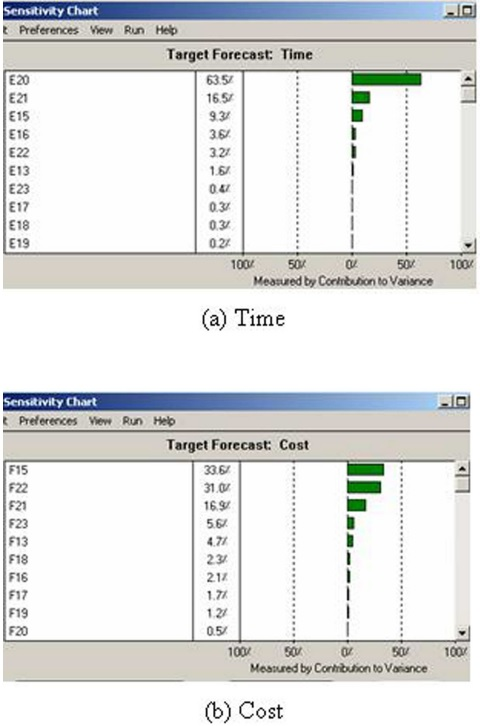
\includegraphics[width=3.34in]{figure/FMANU_MD_05_1107_11.jpg}}
\caption{Example taken from a paper that was held from production because the image quality is poor.  ASME sets figures captions in 8pt, Helvetica Bold.}
\label{fig_example1.jpg}
\end{figure}
%%%%%%%%%%%%%%%% end figure %%%%%%%%%%%%%%%%%%%

In order to place the figure in this template using MSWord, select Insert Picture from File, and use wrapping that is top and bottom. Make sure the figure is 3.25in wide.
 
Figure~`\ref{fig_example1.jpg}
was taken from a recent paper that was held from publication, because the text is fuzzy and unreadable. It was probably obtained by taking a screen shot of the computer output of the authors software. This means the original figure was 72dpi (dots per inch) on a computer screen. There is no way to improve the quality such a low resolution figure.
 
In order to understand how poor the quality of this figure is, please zoom in slightly, say to 200\%.  Notice that while the font of the paper is clear at this size, the font in the figures is fuzzy and blurred.  It is impossible to make out the small symbol beside the numbers along the abscissa of the graph.  Now consider the labels Time and Cost. They are clearly in fonts larger that the text of the article, yet the pixilation or rasterization, associated with low resolution is obvious. This figure must be regenerated at higher resolution to ensure quality presentation.

The poor quality of this figure is immediately obvious on the printed page, and reduces the impact of the research contribution of the paper, and in fact detracts from the perceived quality of the journal itself.



%%%%%%%%%%%%%%%%%%%%%%%%%%%%%%%%%%%%%%%%%%%%%%%%%%%%%%%%%%%%%%%%%%%%%%
\subsection{The 2nd Example of Bad Figure}

%%%%%%%%%%%%%%%% begin figure %%%%%%%%%%%%%%%%%%%
\begin{figure} 
\centerline{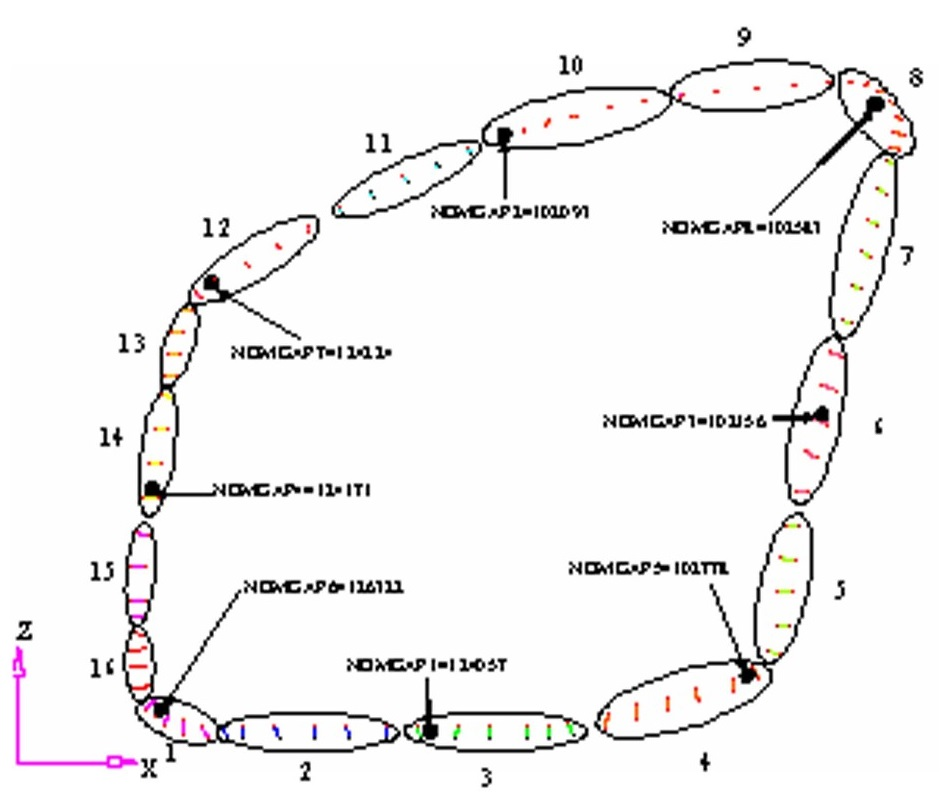
\includegraphics[width=3.34in]{figure/FMANU_MD_05_1272_5.jpg}}
\caption{While this figures is easily readable at a double column width of 6.5in, when it is shrunk to 3.25in column width the text is unreadable. This paper was held from production.}
\label{fig_example2.jpg}
\end{figure}
%%%%%%%%%%%%%%%% end figure %%%%%%%%%%%%%%%%%%%

Figure~\ref{fig_example2.jpg}
demonstrates a common problem that arises when a figure is scaled down fit a single column width of 3.25in.  The original figure had labels that were readable at full size, but become unreadable when scaled to half size.  This figure also suffers from poor resolution as is seen in the jagged lines the ovals that form the chain.

This problem can be addressed by increasing the size of the figure to a double column width of 6.5in, so the text is readable.  But this will not improve the line pixilation, and a large low resolution figure is less desirable than a small one.  This also significantly expands the length of the paper, and may cause it to exceed the JMD nine page limit.  Additional pages require page charges of \$200 per page.  It is best to regenerate the figure at the resolution that ensures a quality presentation.


%%%%%%%%%%%%%%%%%%%%%%%%%%%%%%%%%%%%%%%%%%%%%%%%%%%%%%%%%%%%%%%%%%%%%%
\subsection{The 3rd Example of Bad Figure}
%%%%%%%%%%%%%%%% begin figure %%%%%%%%%%%%%%%%%%%
\begin{figure} 
\centerline{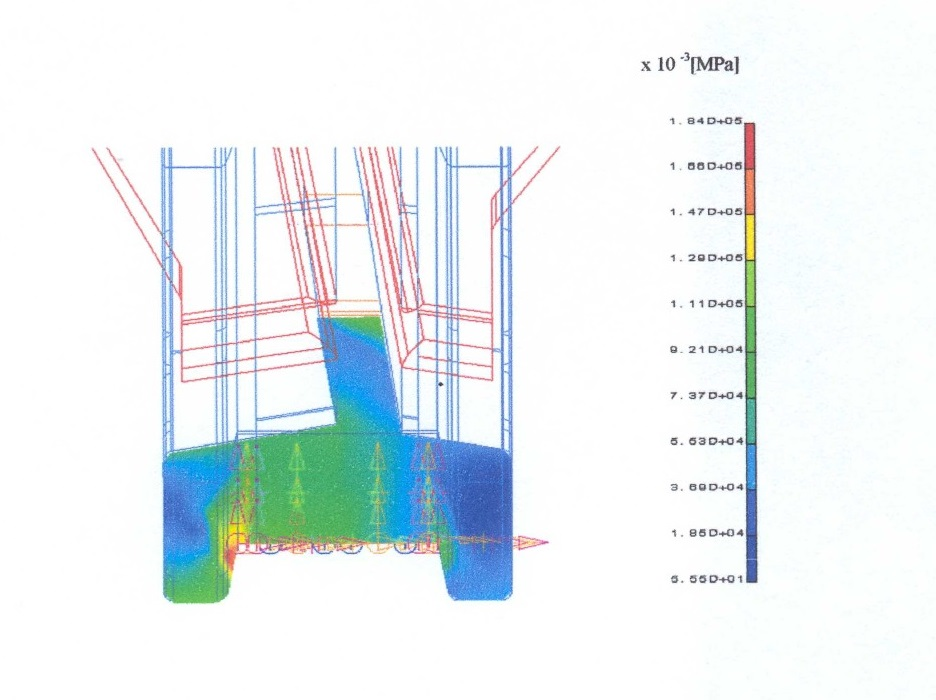
\includegraphics[width=3.25in]{figure/FMANU_MD_04_1274_13.jpg}}
\caption{Another example of a figure with unreadable text.  Even when the paper was expanded to double column width the text as shown in Fig.~\ref{fig_example4.jpg} was of such low quality that the paper was held from production.}
\label{fig_example3.jpg}
\end{figure}
%%%%%%%%%%%%%%%% end figure %%%%%%%%%%%%%%%%%%%

%%%%%%%%%%%%%%%% begin figure %%%%%%%%%%%%%%%%%%%
%%% the maximum width in double column is 6.85in
\begin{figure*} 
\centerline{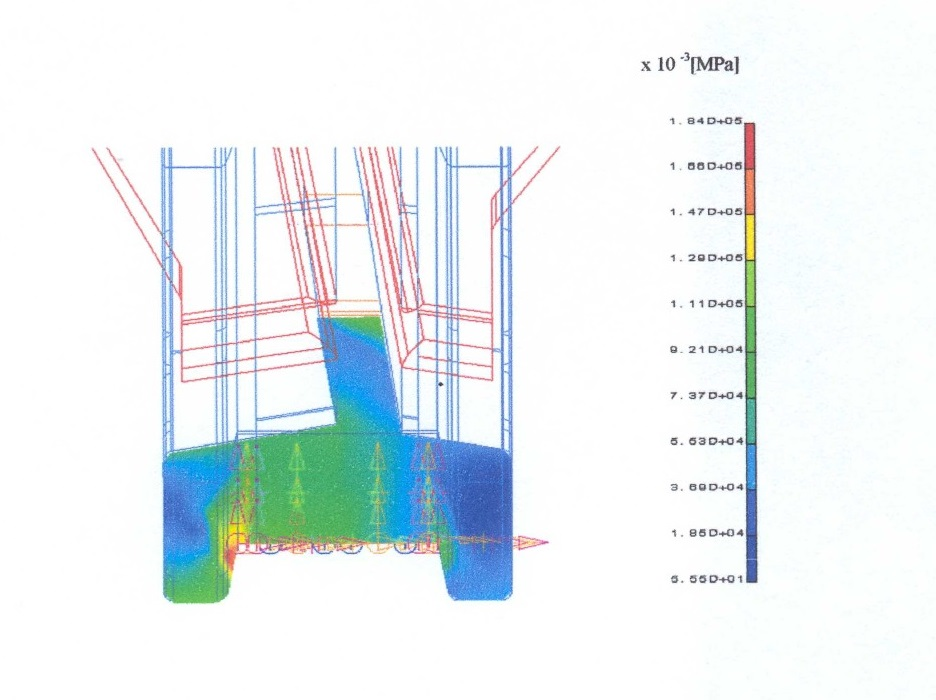
\includegraphics[width=6.85in]{figure/FMANU_MD_04_1274_13.jpg}}
\caption{A figure expanded to double column width the text from Figure~\ref{fig_example3.jpg}}
\label{fig_example4.jpg}
\end{figure*}
%%%%%%%%%%%%%%%% end figure %%%%%%%%%%%%%%%%%%%
An author provided the high resolution image 
in Fig.~\ref{fig_example3.jpg}
that was sized to a single column width of 3.25in.  Upon seeing the poor quality of the text, the publisher scaled the image to double column width as shown in Fig.~\ref{fig_example4.jpg} 
at which point it took half of a page.  The publisher went on to do this for all eight figures generating four pages of figures that the author did not expect. ASME stopped production of the paper even with the larger figures due to the pixilation of the font.

Clearly the text in this figure is unreadable, and it is doubtful that the author can print the output in a way that it is readable.  This is a problem that the author must solve, not the publisher. 

As you might expect, I have many more examples, but in the end the author is the best judge of what is needed in each figure.  ASME simply requires that the image meet a minimum standard for font and line quality, specifically the font should be the appropriate size and not be blurred or pixilated, and that lines should be the appropriate weight and have minimal, preferably no, pixilation or rasterization.


%%%%%%%%%%%%%%%%%%%%%%%%%%%%%%%%%%%%%%%%%%%%%%%%%%%%%%%%%%%%%%%%%%%%%%
\section{Tables}

%%%%%%%%%%%%%%%%%%%%%%%%%%%%%%%%%%%%%%%%%%%%%%%%%%%%%%%%%%%%%%%%%%%%%%
%%%%%%%%%%%%%%% begin table   %%%%%%%%%%%%%%%%%%%%%%%%%%
\begin{table}[t]
\caption{Figure and table captions do not end with a period}
\begin{center}
\label{table_ASME}
\begin{tabular}{c l l}
& & \\ % put some space after the caption
\hline
Example & Time & Cost \\
\hline
1 & 12.5 & \$1,000 \\
2 & 24 & \$2,000 \\
\hline
\end{tabular}
\end{center}
\end{table}
%%%%%%%%%%%%%%%% end table %%%%%%%%%%%%%%%%%%% 
%%%%%%%%%%%%%%%%%%%%%%%%%%%%%%%%%%%%%%%%%%%%%%%%%%%%%%%%%%%%%%%%%%%%%%

All tables should be numbered consecutively  and centered above the table as shown in Table~\ref{table_ASME}. The body of the table should be no smaller than 7 pt.  There should be a minimum two line spaces between tables and text.


%%%%%%%%%%%%%%%%%%%%%%%%%%%%%%%%%%%%%%%%%%%%%%%%%%%%%%%%%%%%%%%%%%%%%%
\section{Citing References}

%%%%%%%%%%%%%%%%%%%%%%%%%%%%%%%%%%%%%%%%%%%%%%%%%%%%%%%%%%%%%%%%%%%%%%
The ASME reference format is defined in the authors kit provided by the ASME.  The format is:

\begin{quotation}
{\em Text Citation}. Within the text, references should be cited in  numerical order according to their order of appearance.  The numbered reference citation should be enclosed in brackets.
\end{quotation}

The references must appear in the paper in the order that they were cited.  In addition, multiple citations (3 or more in the same brackets) must appear as a `` [1-3]''.  A complete definition of the ASME reference format can be found in the  ASME manual \cite{asmemanual}.

The bibliography style required by the ASME is unsorted with entries appearing in the order in which the citations appear. If that were the only specification, the standard {\sc Bib}\TeX\ unsrt bibliography style could be used. Unfortunately, the bibliography style required by the ASME has additional requirements (last name followed by first name, periodical volume in boldface, periodical number inside parentheses, etc.) that are not part of the unsrt style. Therefore, to get ASME bibliography formatting, you must use the \verb+asmems4.bst+ bibliography style file with {\sc Bib}\TeX. This file is not part of the standard BibTeX distribution so you'll need to place the file someplace where LaTeX can find it (one possibility is in the same location as the file being typeset).

With \LaTeX/{\sc Bib}\TeX, \LaTeX\ uses the citation format set by the class file and writes the citation information into the .aux file associated with the \LaTeX\ source. {\sc Bib}\TeX\ reads the .aux file and matches the citations to the entries in the bibliographic data base file specified in the \LaTeX\ source file by the \verb+\bibliography+ command. {\sc Bib}\TeX\ then writes the bibliography in accordance with the rules in the bibliography .bst style file to a .bbl file which \LaTeX\ merges with the source text.  A good description of the use of {\sc Bib}\TeX\ can be found in \cite{latex, goosens} (see how two references are handled?).  The following is an example of how three or more references \cite{latex, asmemanual,  goosens} show up using the \verb+asmems4.bst+ bibliography style file in conjunction with the \verb+asme2ej.cls+ class file. Here are some more \cite{art, blt, ibk, icn, ips, mts, mis, pro, pts, trt, upd} which can be used to describe almost any sort of reference.

%%%%%%%%%%%%%%%%%%%%%%%%%%%%%%%%%%%%%%%%%%%%%%%%%%%%%%%%%%%%%%%%%%%%%%
\section{Conclusions}
The only way to ensure that your figures are presented in the ASME Journal of Mechanical Design in the way you feel is appropriate and meets the requirement for quality presentation is for you to prepare a double column version of the paper in a form similar to that used by the Journal.

This gives you the opportunity to ensure that the figures are sized appropriately, in particular that the labels are readable and match the size of the text in the journal, and that the line weights and resolutions have no pixilation or rasterization.  Poor quality figures are immediately obvious on the printed page, and this detracts from the perceived quality of the journal.

I am pleased to provide advice on how to improve any figure, but this effort must start with a two-column version of the manuscript. Thank you in advance for your patience with this effort, it will ensure quality presentation of your research contributions.



%%%%%%%%%%%%%%%%%%%%%%%%%%%%%%%%%%%%%%%%%%%%%%%%%%%%%%%%%%%%%%%%%%%%%%
\section{Discussions}
This template is not yet ASME journal paper format compliant at this point.
More specifically, the following features are not ASME format compliant.
\begin{enumerate}
\item
The format for the title, author, and abstract in the cover page.
\item
The font for title should be 24 pt Helvetica bold.
\end{enumerate}

\noindent
If you can help to fix these problems, please send us an updated template.
If you know there is any other non-compliant item, please let us know.
We will add it to the above list.
With your help, we shall make this template 
compliant to the ASME journal paper format.


%%%%%%%%%%%%%%%%%%%%%%%%%%%%%%%%%%%%%%%%%%%%%%%%%%%%%%%%%%%%%%%%%%%%%%
\begin{acknowledgment}
ASME Technical Publications provided the format specifications for the Journal of Mechanical Design, though they are not easy to reproduce.  It is their commitment to ensuring quality figures in every issue of JMD that motivates this effort to have authors review the presentation of their figures.  

Thanks go to D. E. Knuth and L. Lamport for developing the wonderful word processing software packages \TeX\ and \LaTeX. We would like to thank Ken Sprott, Kirk van Katwyk, and Matt Campbell for fixing bugs in the ASME style file \verb+asme2ej.cls+, and Geoff Shiflett for creating 
ASME bibliography stype file \verb+asmems4.bst+.
\end{acknowledgment}

%%%%%%%%%%%%%%%%%%%%%%%%%%%%%%%%%%%%%%%%%%%%%%%%%%%%%%%%%%%%%%%%%%%%%%
% The bibliography is stored in an external database file
% in the BibTeX format (file_name.bib).  The bibliography is
% created by the following command and it will appear in this
% position in the document. You may, of course, create your
% own bibliography by using thebibliography environment as in
%
% \begin{thebibliography}{12}
% ...
% \bibitem{itemreference} D. E. Knudsen.
% {\em 1966 World Bnus Almanac.}
% {Permafrost Press, Novosibirsk.}
% ...
% \end{thebibliography}

% Here's where you specify the bibliography style file.
% The full file name for the bibliography style file 
% used for an ASME paper is asmems4.bst.
\bibliographystyle{asmems4}

% Here's where you specify the bibliography database file.
% The full file name of the bibliography database for this
% article is asme2e.bib. The name for your database is up
% to you.
\bibliography{asme2e}

%%%%%%%%%%%%%%%%%%%%%%%%%%%%%%%%%%%%%%%%%%%%%%%%%%%%%%%%%%%%%%%%%%%%%%
\appendix       %%% starting appendix
\section*{Appendix A: Head of First Appendix}
Avoid Appendices if possible.

%%%%%%%%%%%%%%%%%%%%%%%%%%%%%%%%%%%%%%%%%%%%%%%%%%%%%%%%%%%%%%%%%%%%%%
\section*{Appendix B: Head of Second Appendix}
\subsection*{Subsection head in appendix}
The equation counter is not reset in an appendix and the numbers will
follow one continual sequence from the beginning of the article to the very end as shown in the following example.
\begin{equation}
a = b + c.
\end{equation}

\end{document}
